

\tikzset{every picture/.style={line width=0.75pt}} %set default line width to 0.75pt        

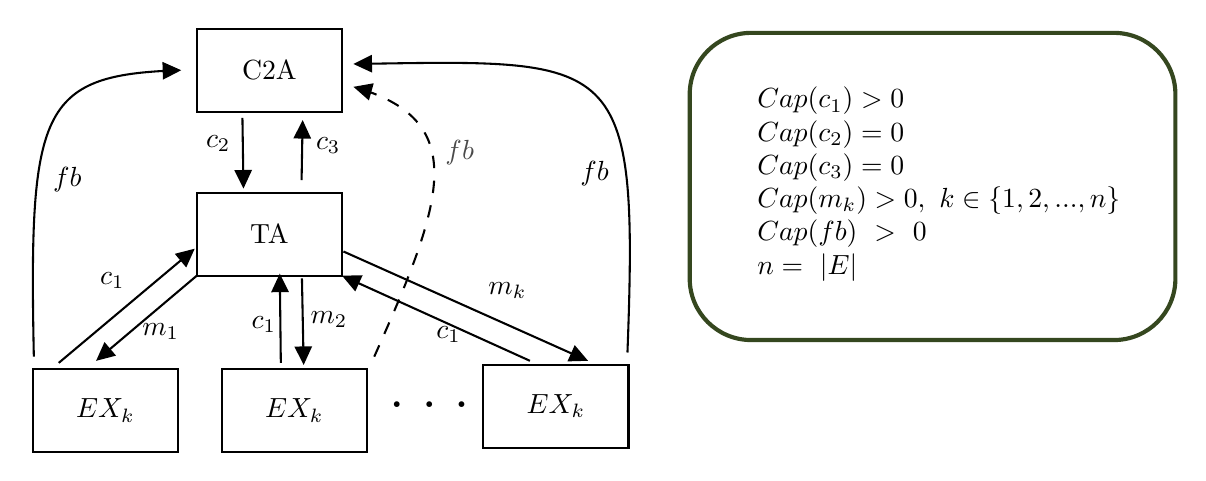
\begin{tikzpicture}[x=0.75pt,y=0.75pt,yscale=-1,xscale=1]
%uncomment if require: \path (0,229); %set diagram left start at 0, and has height of 229

%Shape: Rectangle [id:dp7793135649662085] 
\draw   (105,88) -- (175,88) -- (175,128) -- (105,128) -- cycle ;
%Shape: Rectangle [id:dp8388066725390221] 
\draw   (105,9) -- (175,9) -- (175,49) -- (105,49) -- cycle ;
%Shape: Rectangle [id:dp48691256180587716] 
\draw   (26,173) -- (96,173) -- (96,213) -- (26,213) -- cycle ;
%Straight Lines [id:da3337977868298102] 
\draw    (127,52) -- (127.46,83) ;
\draw [shift={(127.5,86)}, rotate = 269.15999999999997] [fill={rgb, 255:red, 0; green, 0; blue, 0 }  ][line width=0.08]  [draw opacity=0] (8.93,-4.29) -- (0,0) -- (8.93,4.29) -- cycle    ;
%Straight Lines [id:da7136052167478543] 
\draw    (155.67,129.33) -- (156.44,168) ;
\draw [shift={(156.5,171)}, rotate = 268.85] [fill={rgb, 255:red, 0; green, 0; blue, 0 }  ][line width=0.08]  [draw opacity=0] (8.93,-4.29) -- (0,0) -- (8.93,4.29) -- cycle    ;
%Straight Lines [id:da1199439366931846] 
\draw    (38.5,170) -- (101.7,116.93) ;
\draw [shift={(104,115)}, rotate = 499.98] [fill={rgb, 255:red, 0; green, 0; blue, 0 }  ][line width=0.08]  [draw opacity=0] (8.93,-4.29) -- (0,0) -- (8.93,4.29) -- cycle    ;
%Rounded Rect [id:dp3574279176331121] 
\draw  [color={rgb, 255:red, 53; green, 71; blue, 31 }  ,draw opacity=1 ][line width=1.5]  (342.5,40.6) .. controls (342.5,24.25) and (355.75,11) .. (372.1,11) -- (546.9,11) .. controls (563.25,11) and (576.5,24.25) .. (576.5,40.6) -- (576.5,129.4) .. controls (576.5,145.75) and (563.25,159) .. (546.9,159) -- (372.1,159) .. controls (355.75,159) and (342.5,145.75) .. (342.5,129.4) -- cycle ;
%Curve Lines [id:da7275055445236782] 
\draw    (26.5,167) .. controls (24.03,48.2) and (29.39,31.33) .. (95.48,29.06) ;
\draw [shift={(97.5,29)}, rotate = 538.3199999999999] [fill={rgb, 255:red, 0; green, 0; blue, 0 }  ][line width=0.08]  [draw opacity=0] (8.93,-4.29) -- (0,0) -- (8.93,4.29) -- cycle    ;
%Shape: Rectangle [id:dp8070909053866772] 
\draw   (243,171) -- (313,171) -- (313,211) -- (243,211) -- cycle ;
%Shape: Rectangle [id:dp18131918632628874] 
\draw   (117,173) -- (187,173) -- (187,213) -- (117,213) -- cycle ;
%Straight Lines [id:da4580469739796602] 
\draw    (145.5,170) -- (145.03,130) ;
\draw [shift={(145,127)}, rotate = 449.33] [fill={rgb, 255:red, 0; green, 0; blue, 0 }  ][line width=0.08]  [draw opacity=0] (8.93,-4.29) -- (0,0) -- (8.93,4.29) -- cycle    ;
%Straight Lines [id:da23459308482895536] 
\draw    (265.5,169) -- (177.73,129.24) ;
\draw [shift={(175,128)}, rotate = 384.37] [fill={rgb, 255:red, 0; green, 0; blue, 0 }  ][line width=0.08]  [draw opacity=0] (8.93,-4.29) -- (0,0) -- (8.93,4.29) -- cycle    ;
%Straight Lines [id:da9340034396500284] 
\draw    (175.67,116.33) -- (290.76,167.78) ;
\draw [shift={(293.5,169)}, rotate = 204.07999999999998] [fill={rgb, 255:red, 0; green, 0; blue, 0 }  ][line width=0.08]  [draw opacity=0] (8.93,-4.29) -- (0,0) -- (8.93,4.29) -- cycle    ;
%Straight Lines [id:da26523318096149495] 
\draw    (105,128) -- (58.79,167.06) ;
\draw [shift={(56.5,169)}, rotate = 319.78999999999996] [fill={rgb, 255:red, 0; green, 0; blue, 0 }  ][line width=0.08]  [draw opacity=0] (8.93,-4.29) -- (0,0) -- (8.93,4.29) -- cycle    ;
%Curve Lines [id:da641554832923748] 
\draw    (312.5,165) .. controls (317.97,20.72) and (308.59,23.96) .. (182.41,25.97) ;
\draw [shift={(180.5,26)}, rotate = 359.1] [fill={rgb, 255:red, 0; green, 0; blue, 0 }  ][line width=0.08]  [draw opacity=0] (8.93,-4.29) -- (0,0) -- (8.93,4.29) -- cycle    ;
%Curve Lines [id:da09438027167232854] 
\draw  [dash pattern={on 4.5pt off 4.5pt}]  (190.5,167) .. controls (223.5,93.12) and (237.09,54.18) .. (183.02,37.74) ;
\draw [shift={(180.5,37)}, rotate = 375.68] [fill={rgb, 255:red, 0; green, 0; blue, 0 }  ][line width=0.08]  [draw opacity=0] (8.93,-4.29) -- (0,0) -- (8.93,4.29) -- cycle    ;
%Straight Lines [id:da9905404427936819] 
\draw    (155.95,56) -- (155.5,82) ;
\draw [shift={(156,53)}, rotate = 90.99] [fill={rgb, 255:red, 0; green, 0; blue, 0 }  ][line width=0.08]  [draw opacity=0] (8.93,-4.29) -- (0,0) -- (8.93,4.29) -- cycle    ;

% Text Node
\draw (140,29) node   [align=left] {C2A};
% Text Node
\draw (140,108) node   [align=left] {TA};
% Text Node
\draw (61,193) node    {$EX_{k}$};
% Text Node
\draw (64.33,130.33) node    {$c_{1}$};
% Text Node
\draw (168.67,149) node    {$m_{2}$};
% Text Node
\draw (115.33,64.33) node    {$c_{2}$};
% Text Node
\draw (462.5,84) node    {$ \begin{array}{l}
Cap( c_{1})  >0\\
Cap( c_{2}) =0\\
Cap( c_{3}) =0\\
Cap( m_{k})  >0,\ k\in \{1,2,...,n\}\\
Cap( fb) \  >\ 0\\
n=\ |E|\ 
\end{array}$};
% Text Node
\draw (42.67,81.67) node    {$fb$};
% Text Node
\draw (278,191) node    {$EX_{k}$};
% Text Node
\draw (152,193) node    {$EX_{k}$};
% Text Node
\draw (217,190) node  [font=\Large] [align=left] {\textbf{. . .}};
% Text Node
\draw (254.67,135) node    {$m_{k}$};
% Text Node
\draw (87.67,155) node    {$m_{1}$};
% Text Node
\draw (137.33,151.33) node    {$c_{1}$};
% Text Node
\draw (226.33,156.33) node    {$c_{1}$};
% Text Node
\draw (296.67,78.67) node    {$fb$};
% Text Node
\draw (231.67,68.67) node  [color={rgb, 255:red, 74; green, 74; blue, 74 }  ,opacity=1 ]  {$fb$};
% Text Node
\draw (168.33,65.33) node    {$c_{3}$};


\end{tikzpicture}